\documentclass[screen, aspectratio=43]{beamer}
\usepackage[T1]{fontenc}
\usepackage[utf8]{inputenc}
\usepackage{natbib}
\bibliographystyle{plain}
\usepackage{tikz}
\usepackage{graphicx}
\usepackage{subfig}
\captionsetup[subfigure]{labelformat=empty}
\captionsetup[figure]{labelformat=empty}
\usetikzlibrary{tikzmark,positioning,calc,arrows}
%\usetikzlibrary{shapes,arrows,calc,positioning,shadows,fillbetween}
\usepackage{tcolorbox}
\usepackage[absolute,overlay]{textpos}
\usepackage{multimedia}
\definecolor{re}{rgb}{0.8500, 0.3250, 0.0980}
\definecolor{ye}{rgb}{    0.9290    0.6940    0.1250}
\newtcolorbox{mybox}[2]{colback=white, colframe=ntnublue,
  fonttitle=\large, title=#1, text height=#2, fontupper=\color{black}\footnotesize}%
\newtcolorbox{myboxRed}[2]{colback=white, colframe=re,
  fonttitle=\large, title=#1, text height=#2, fontupper=\color{black}\footnotesize}%

\newcommand{\myitemmark}{\raisebox{.75ex}{\scalebox{.6}{\protect\colorbox{ntnublue}{\protect}}}}
\newenvironment{prettyList}
{
  \begin{list}{\myitemmark}{\leftmargin=1.5em \itemindent=0em} 
}
{
  \end{list}
}

\DeclareMathOperator{\eff}{eff}
\DeclareMathOperator{\dd}{d}
\newcommand{\mat}[1]{\boldsymbol{#1}}


% Use the NTNU-temaet for beamer 
% \usetheme[style=ntnu|simple|vertical|horizontal, language=bm|nn|en]{ntnu2015}
\usetheme[style=ntnu,language=en]{ntnu2015}
 
\title[Short title]{Implementation of a Solvent Model Using MRST}
%\subtitle{Subtitle if you want}
\author[Ø.S. Klemetsdal]{Øystein Strengehagen Klemetsdal}
\institute[NTNU]{Department of Mathematical Sciences, NTNU}
%\date{1 January 1970}
\date{} % To have an empty date

\begin{document}

% Special title page command to get a different background
\ntnutitlepage

\begin{frame}
  \frametitle{Outline}
  \tableofcontents
\end{frame}

\section{Introduction}

\begin{frame}
  \frametitle{Outline}
  \tableofcontents[currentsection]
\end{frame}


\begin{frame}
  \frametitle{Miscible flooding}
  \vspace{0.5cm}
  Proven, economically viable recovery technique \cite{petroWiki2017Misc}
  \begin{prettyList}
  \item Recovers much of the trapped oil after a waterflood
  \item Displaces oil in regions poorly swept by water due to gravity
  \item May be used in combination with CO$_2$ storage
  \item Three main injection strategies: slug injection, water-alternating-gas (WAG) and
    gravity-stable injection
  \end{prettyList}
  \begin{figure}[h]
    \centering
    \subfloat[$S_o$ after waterflood]{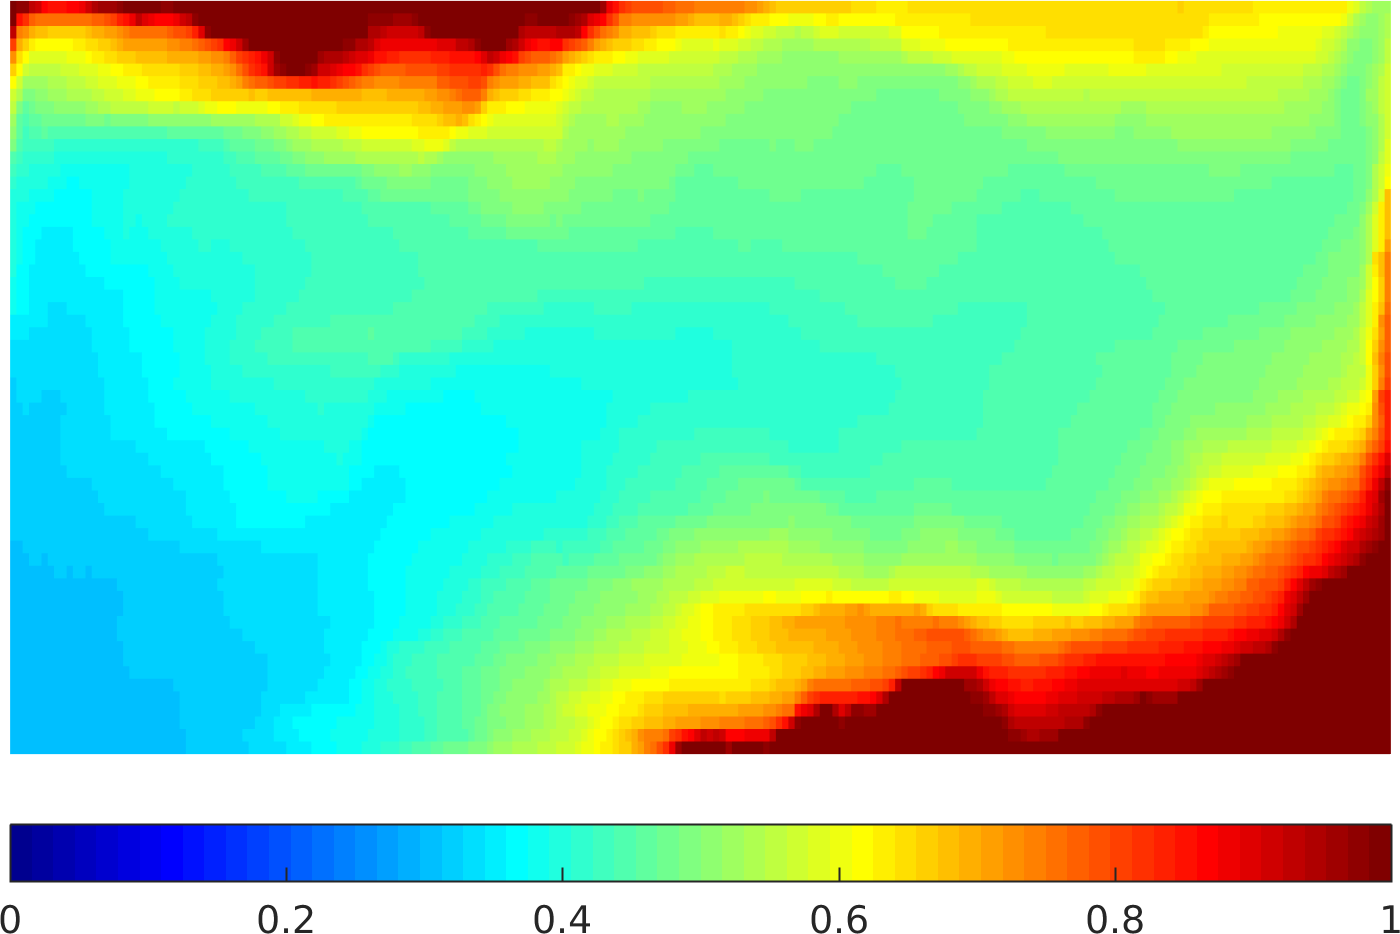
\includegraphics[width = 0.4\textwidth]{figures/misc/wagEx1}}\hspace{1em}
    \subfloat[$S_o$ after waterflood + WAG]{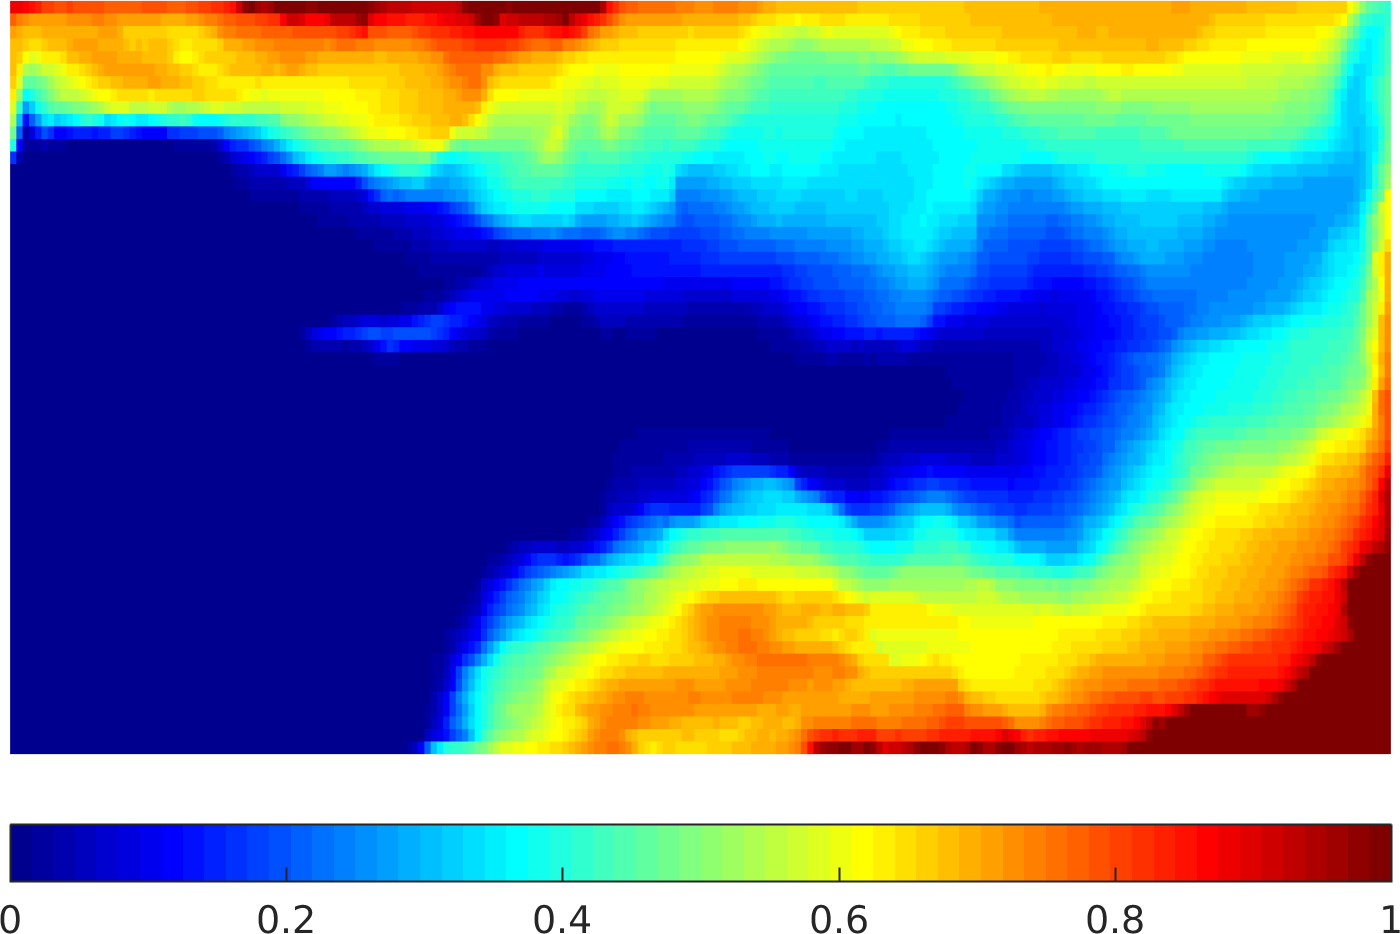
\includegraphics[width = 0.4\textwidth]{figures/misc/wagEx2}}
  \end{figure}
\end{frame}

\begin{frame}
  \frametitle{Physics of miscible flooding}
  \only<1>{
    \begin{columns}
      \begin{column}{0.65\textwidth}
        \begin{prettyList}
        \item Miscible displacement: No interface between injected fluid and reservoir oil
        \item Fully miscible displacement: Injected solvent displaces \emph{all}
          residual oil from invaded pores
        \item Most physical gases do not form a completely miscible system when combined
          with reservoir oil
        \end{prettyList}
      \end{column}
      \begin{column}{0.3\textwidth}
        \begin{figure}[h]
          \centering
          \includegraphics[height=0.85\textheight]{figures/misc/miscible}
        \end{figure}
      \end{column}
    \end{columns}
  }
  \only<2->{
    \begin{columns}
      \begin{column}{0.7\textwidth}
        Key physical phenomena \cite{schlumberger2013eclipse}
        \begin{prettyList}
        \item High adverse \textcolor{re}{mobility ratio} \\ \hspace{0.5cm} $\Rightarrow$ Unstable flow, viscous fingers
        \item Large \textcolor{re}{density differences} \\ \hspace{0.5cm} $\Rightarrow$ Gravitational fingers
        \item The growth of both types of fingers is dampened by \textcolor{re}{mixing}
        \item A good solvent model should account for \textcolor{re}{all these effects}
        \end{prettyList}
      \end{column}
      \begin{column}{0.25\textwidth}
        \begin{figure}[h]
          \centering
          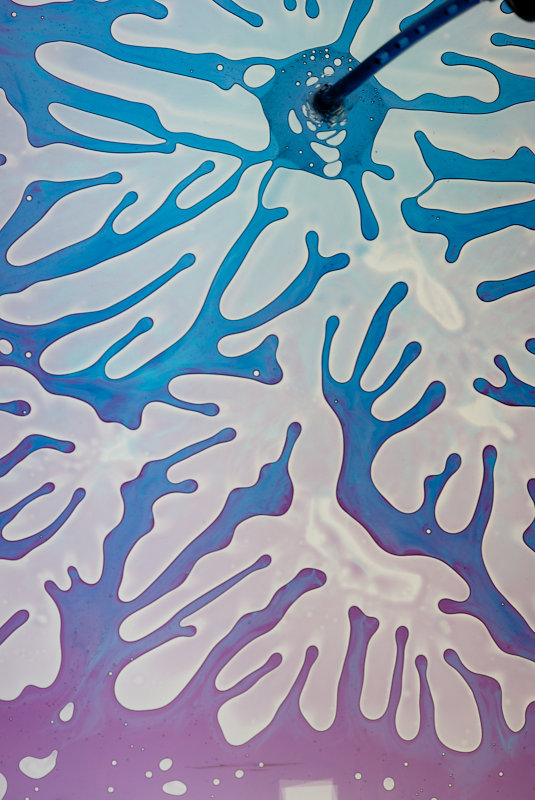
\includegraphics[trim={0 0 5cm 0}, clip, width = \textwidth]{figures/misc/mf}
          \caption{\scriptsize Viscous fingers in a Hele-Shaw cell
            {\tiny \url{http://n-e-r-v-o-u-s.com}}}
%          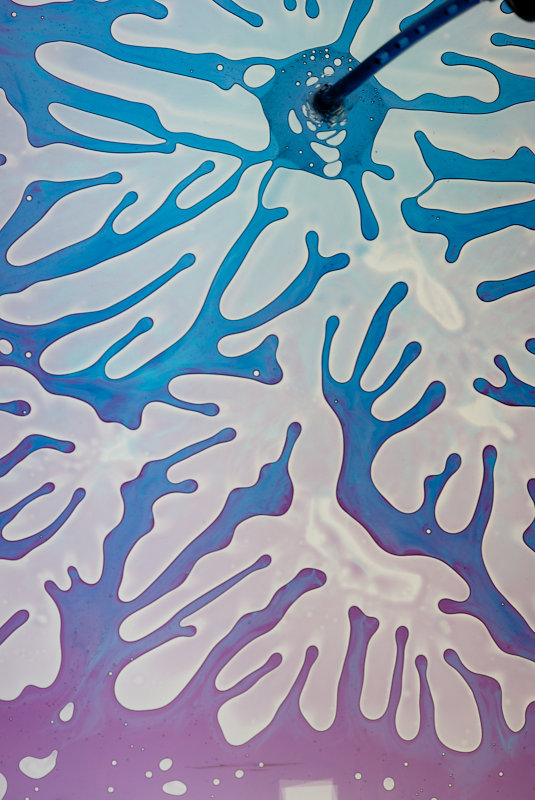
\includegraphics[width = \textwidth]{figures/misc/mf}
        \end{figure}
      \end{column}
    \end{columns}
  }
\end{frame}

\section{Model formulation}

\begin{frame}
  \frametitle{Outline}
  \tableofcontents[currentsection]
\end{frame}

\begin{frame}
  \frametitle{First attempts}
  Based on direct solution of convection-diffusion equations \cite{peaceman1962numerical}
  \begin{equation*}
    c_t + \nabla \cdot (\vec v c)  = \nabla \cdot (D\nabla c )
  \end{equation*}
  On coarse grids:
  \begin{list}{\myitemmark}{\leftmargin=1.5em \itemindent=0em} 
  \item Fails to capture the fine-scale structure of the fingers
  \item True mixing masked by numerical diffusion
  \end{list}
  $\Rightarrow$ Unacceptably high grid resolution
\end{frame}

\begin{frame}
  \frametitle{Model assumptions}
  \vspace{0.5cm}
  We consider the model implemented in ECLIPSE \cite{geoquest2002eclipse}
  \begin{prettyList}
  \item Separate solvent phase $\Rightarrow$ avoid fully compositional formulation
  \end{prettyList}
  % \begin{prettyList}
  % \item Two extreme cases:
  %   \begin{enumerate}
  %   \item Only reservoir gas and oil: Immiscible
  %   \item Only solvent gas and reservoir oil: Miscible in all proportions
  %   \end{enumerate}
  % \item Interpolate in regions containing both dry gas and
  %   solvent
  % \end{prettyList}
  \begin{figure}[h]
    \centering
    \includegraphics[width=\textwidth]{figures/misc/miscible2}
  \end{figure}
  
\end{frame}

\begin{frame}
  \frametitle{Governing equations}
  \begin{prettyList}
  \item \textcolor{re}{One extra} pseudo-component $\Rightarrow$ \textcolor{re}{One extra} conservation equation
  \begin{align*}
    \begin{aligned}
      \partial_t(\phi \only<2>{\textcolor{ye}}{\rho_\alpha} S_\alpha)
      + \nabla \cdot (\only<2>{\textcolor{ye}}{\rho_\alpha} \vec v_\alpha) = \only<2>{\textcolor{ye}}{\rho_\alpha} q_\alpha \\
    \vec v_\alpha = -\frac{\only<2>{\textcolor{ye}}{k_{r\alpha}}}{\only<2>{\textcolor{ye}}{\mu_\alpha}}K
    \left(\nabla p_\alpha - \only<2>{\textcolor{ye}}{\rho_\alpha} g \nabla z\right)
  \end{aligned} \quad \quad  \alpha \in \{w, o, g, \textcolor{re}{s}\}
  \end{align*}
\item Solvent affects the \only<2>{\textcolor{ye}}{relative permeabilities}, \only<2>{\textcolor{ye}}{viscosities} and
  \only<2>{\textcolor{ye}}{densities}
\item Effective quantities are derived from the Todd-Longstaff model for miscible flooding \cite{todd1972development}
  \end{prettyList}
\end{frame}

\begin{frame}
  \frametitle{Relative permeabilities}
  \begin{align*}
    k_{r \alpha,\textcolor{re}{\only<1>{i}\only<2>{m}}} = \underbrace{m_\alpha \left(\frac{S_\alpha}{S_g + S_s}\right)}_{\tikzmark{malpha}}
    \underbrace{k_{rgT,\textcolor{re}{\only<1>{i}\only<2>{m}}}(S_o, S_g, S_s)}_{\tikzmark{krgT}},
    \quad \alpha \in \{g, s\}
  \end{align*}
  \begin{tikzpicture}[remember picture,overlay]
    \draw [bend left, <-, line width = 1pt]($({pic cs:malpha})+(0,6pt)$) |- ++(-1em,-2ex)
    node[rectangle, anchor=east,font=\small, text width = 2.5cm, align = center, fill = ntnublue!20]
    {\scriptsize Relperm multiplier};
    \draw [<-, line width = 1pt]($({pic cs:krgT})+(0,6pt)$) |- ++(1em,-3.3ex)
    node[rectangle, anchor=west,font=\small, text width = 2.5cm, align = center, fill = ntnublue!20]
    {\scriptsize Total gas relperm};
  \end{tikzpicture}%
  \\\vspace{0.5cm}
  \begin{columns}
    \begin{column}{0.5\textwidth}
      \only<1>{\begin{myboxRed}{\centering Immiscible case ($i$)}{0.3\textheight}}
        \only<2>{\begin{mybox}{\centering Immiscible case ($i$)}{0.3\textheight}}
          \vspace{0.4cm}
        \begin{align*}
          k_{r o,i} & = k_{ro}(S_o) \\
          k_{rgT,i} & = k_{rg}(S_g + S_s)
        \end{align*}
      \only<1>{\end{myboxRed}}
      \only<2>{\end{mybox}}
    \end{column}
    \begin{column}{0.5\textwidth}
      \only<1>{\begin{mybox}{\centering Miscible case ($m$)}{0.3\textheight}}
      \only<2>{\begin{myboxRed}{\centering Miscible case ($m$)}{0.3\textheight}}
        \begin{align*}
          k_{r o,m} & = \frac{S_o}{S_n}k_{rn}(S_n) \\
          k_{rgT,m} & = \frac{S_g + S_s}{S_n}k_{rn}(S_n) \\
          S_n & = S_o + S_g + S_s
        \end{align*}
      \only<1>{\end{mybox}}
      \only<2>{\end{myboxRed}}
    \end{column}
  \end{columns}
\end{frame}

\begin{frame}
  \frametitle{Transition between miscible and immiscible conditions}
  \only<1>{
    \begin{prettyList}
    \item Determined by miscibility function
      \begin{equation*}
        \textcolor{re}{M} = \underbrace{M_S\left(\frac{S_s}{S_g + S_s}\right)}_{\tikzmark{Ms}} M_p\tikzmark{Mp}(p) \in [0,1]
      \end{equation*}
      \begin{tikzpicture}[remember picture,overlay]
        \draw [bend left, <-, line width = 1pt]($({pic cs:Ms})+(0,7pt)$) |- ++(-1em,-2ex)
        node[rectangle, anchor=east,font=\small, text width = 3cm, align = center, fill = ntnublue!20]
        {\scriptsize Saturation dependence};
        \draw [bend left, <-, line width = 1pt]($({pic cs:Mp})-(0,5pt)$) |- ++(1em,-4.3ex)
        node[rectangle, anchor=west,font=\small, text width = 3cm, align = center, fill = ntnublue!20]
        {\scriptsize Pressure dependence};
      \end{tikzpicture}%
      \\\vspace{0.3cm}
    \item Two-step transition:
      \begin{enumerate}
      \item Interpolate residual saturations, and use these as new endpoints in the relative permeabilities
        \begin{align*}
          S_{\alpha r} = S_{\alpha r,m}\textcolor{re}{M} + S_{\alpha r,i}(1-\textcolor{re}{M}), \quad \alpha \in \{o,g\}
        \end{align*}
      \item Interpolate relative permeabilities
        \begin{align*}
          k_{r \alpha} = k_{r\alpha,m}\textcolor{re}{M} + k_{r\alpha,i}(1-\textcolor{re}{M}), \quad \alpha \in \{o,gT\}
        \end{align*}
      \end{enumerate}
    \end{prettyList}
  }
  \only<2>{
    \begin{figure}[h]
      \vspace{0.5cm}
      \centering
      \begin{tikzpicture}
        \node[anchor=south west,inner sep=0] at (0,0) {
          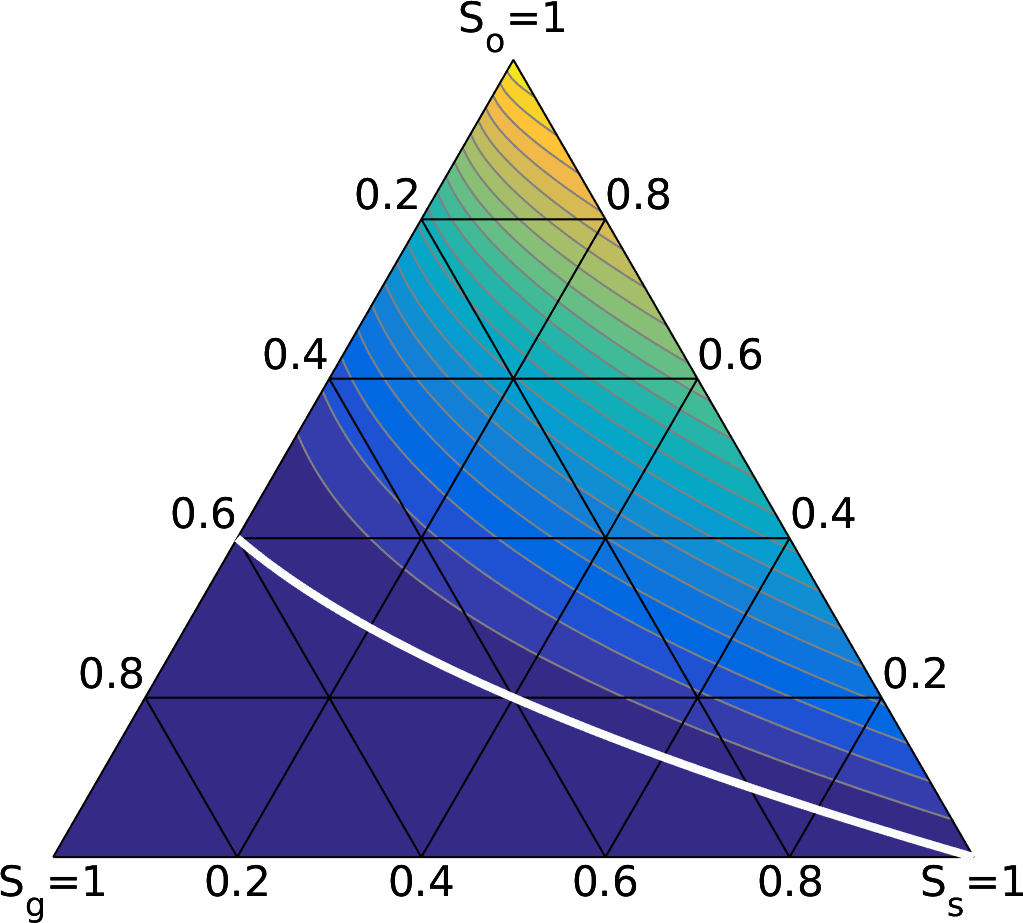
\includegraphics[width = 0.6\textwidth]{figures/misc/krO.png}};
        \node[rotate = 60] at (1,3.5) {Immiscible regime};
        \node[rotate = -60] at (5.8,3.5) {Miscible regime};
        \node[rotate = -20, color = white] at (3.2,1.3) { Residual oil saturation};
      \end{tikzpicture}
    \end{figure}
  }
  \only<3>{
    \vspace{0.5cm}
    \begin{figure}[h]
      \centering
      \includegraphics[width = 0.9\textwidth]{figures/misc/ternearyAll}
    \end{figure}
  }
\end{frame}


\begin{frame}
  \frametitle{Viscosities}
  \vfill
  Effective viscosities are defined as
  \begin{align*}
    \mu_{o, \eff} = \mu\tikzmark{muo}_o^{1-\only<2>{\textcolor{re}}{\omega}}\only<3>{\textcolor{re}}{\mu\tikzmark{mumos}_{mos}}^{\only<2>{\textcolor{re}}{\omega}}
  \end{align*}
  \begin{tikzpicture}[remember picture,overlay]
    \draw [bend left, <-, line width = 1pt]($({pic cs:muo})-(0,5pt)$) |- ++(-1em,-3ex)
    node[rectangle, anchor=east,font=\small, text width = 2.4cm, align = center, fill = ntnublue!20]
    {\scriptsize Pure oil viscosity};
    \draw [bend left, <-, line width = 1pt]($({pic cs:mumos})-(0,5pt)$) |- ++(1em,-3ex)
    node[rectangle, anchor=west,font=\small, text width = 3.6cm, align = center, fill = ntnublue!20]
    {\scriptsize Fully mixed $o+s$ viscosity};
  \end{tikzpicture}%
  \\\vspace{0.5cm}
  % Effective viscosities determined by Todd-Longstaff model:
  % \begin{equation*}
  %   \mu_{o, \eff} = \mu_o^{1-\omega}\mu_{mos}^\omega
  % \end{equation*}
  % \vspace{0.2cm}
  \begin{prettyList}
  \item Degree of mixing controlled by mixing parameter:
    \begin{equation*}
      \text{no mixing} \leftrightarrow 0 \leq \only<2>{\textcolor{re}}{\omega} \leq 1 \leftrightarrow \text{full mixing}
    \end{equation*}
  \item Fully mixed viscosities determined by $1/4$th power mixing rule:
    \begin{align*}
      \only<3>{\textcolor{re}}{\mu_{mos}} = \frac{\mu_o \mu_s}{\left(\frac{S_o}{S_o + S_s}\mu_s^{1/4} +
      \frac{S_s}{S_o + S_s}\mu_o^{1/4}\right)^4}
    \end{align*}
  \end{prettyList}
      
  % \begin{mybox}{Todd-Longstaff model}{0.3\textheight}
  %   \vspace{0.1cm}
  %   \begin{description}
  %   \item[$\omega$] Mixing parameter $\in [0\leftrightarrow$ no mixing, $1 \leftrightarrow$ full mixing$]$
  %   \item[$\mu_{mos}$] Determined by 4th power mixing rule:
  %     \begin{align*}
  %       \mu_{mos} = \frac{\mu_o \mu_s}{\left(\frac{S_o}{S_o + S_s}\mu_s^{1/4} +
  %       \frac{S_s}{S_o + S_s}\mu_o^{1/4}\right)^4}
  %     \end{align*}
  %   %   $ = \frac{\mu_s \mu_g}{\left(\frac{S_s'}{S_{sg}'}\mu_g^{1/4} +
  %   %       \frac{S_g'}{S_{sg}'}\mu_s^{1/4}\right)^4}$
  %   % \item[$\mu_{m}$] Fully mixed $o +s + g$ viscosity \\
  %   %   \hfill $ = \frac{\mu_o \mu_s \mu_g}{\left(\frac{S_o'}{S_{n}'}(\mu_s\mu_g)^{1/4}
  %   %       + \frac{S_s'}{S_{n}'}(\mu_o\mu_g)^{1/4}
  %   %       + \frac{S_g'}{S_{n}'}(\mu_o\mu_s)^{1/4}\right)^4}$
  %   \end{description}
  % \end{mybox}

\end{frame}

\begin{frame}
  \frametitle{Densities}
  \vfill
  Mixed densities are interpolated using the saturation fractions
  \begin{align*}
    \rho_{o,\eff} & = \rho_o\only<1>{\frac{S_o}{S_o + S_s}}
                    \only<2>{\textcolor{re}{\left[\frac{S_o}{S_o + S_s}\right]_{\eff}}}
                    + \rho_s\left(1 - \only<1>{\frac{S_o}{S_o + S_s}}
                    \only<2>{\textcolor{re}{\left[\frac{S_o}{S_o + S_s}\right]_{\eff}}}\right)
  \end{align*}
  \begin{prettyList}
  \item To be consistent with the viscosity model, we use \emph{effective} saturation fractions
  \begin{align*}
    \only<1>{\mu_{mos}}\only<2>{\textcolor{re}{\mu_{o,\eff}}}
    = \frac{\mu_o \mu_s}{\left(\only<1>{\frac{S_o}{S_o + S_s}}
    \only<2>{\textcolor{re}{\left[\frac{S_o}{S_o + S_s}\right]_{\eff}}}\mu_s^{1/4} +
    \left(1-\only<1>{\frac{S_o}{S_o + S_s}}
    \only<2>{\textcolor{re}{\left[\frac{S_o}{S_o + S_s}\right]_{\eff}}}\right)\mu_o^{1/4}\right)^4}
    % \left[\frac{S_o}{S_o + S_s}\right]_{\eff} = \frac{(\mu_o/\mu_s)^{1/4} - (\mu_o/\mu_{o,\eff})^{1/4}}{(\mu_o/\mu_s)^{1/4} - 1}
    % \mu_{mos} = \frac{\mu_o \mu_s}{\left(\        {S_o}{S_o + S_s}\mu_s^{1/4} +
    % \frac{S_s}{S_o + S_s}\mu_o^{1/4}\right)^4}
  \end{align*}
\end{prettyList}
  
\end{frame}

% \begin{frame}
%   \lstinputlisting[caption = ,firstline =  5, lastline = 10]{../code/FourPhaseSolvent/computeRelPermSolvent.m}
%   \lstinputlisting[caption = ,firstline = 5, lastline = 10]{../code/FourPhaseSolvent/computeViscositiesAndDensities.m}
% \end{frame}


\section{Implementation}

\begin{frame}
  \frametitle{Outline}
  \tableofcontents[currentsection]
\end{frame}

\begin{frame}
  \frametitle{Finite volume discretization}

  \begin{columns}
    \begin{column}{0.6\textwidth}
        Introduce grid of cells $C_i$, and integrate over each cell in space:
      \begin{align*}
        & \bigl[(\phi b_\alpha S_\alpha)_i^{n+1} - (\phi b_\alpha
          S_\alpha)_i^n\bigr] \\
        & + \frac{\Delta t}{V_i}\sum\nolimits_j \only<2>{\textcolor{re}}{|F_{ij}| (b_\alpha
          \vec{v}_\alpha\cdot\vec{n})_{ij}}^{n+1} = \frac{\Delta t}{V_i} (b_\alpha q_\alpha)_i^{n+1}
      \end{align*}
    \end{column}
    \begin{column}{0.3\textwidth}
      \begin{figure}[h]
        \centering
        \includegraphics[width = \textwidth]{figures/misc/tpfa}
      \end{figure}
    \end{column}
  \end{columns}

  \begin{overlayarea}{\textwidth}{0.4\textheight}
    \only<1>{
      \vspace{0.5cm}
      \begin{prettyList}
      \item Backward differences in time
      \item Inverse formation volume factor $b_\alpha = \frac{\rho_\alpha}{\rho_\alpha^s}$ 
      \end{prettyList}
    }
    \only<2>{
      \begin{prettyList}
      \item Mass fluxes approximated using two-point approximation
      \end{prettyList}
      \begin{equation*}
        \textcolor{re}{|F_{ij}|(b_\alpha \vec v_\alpha\cdot\vec n)_{ij}} \approx
        \underbrace{(b_\alpha\lambda_\alpha)_{ij}}_{\tikzmark{up}}
        \Bigl[ T_{ij}(p_i - p_j) -
        \underbrace{(b_\alpha)_{ij}}_{\tikzmark{av}}
        \rho_\alpha^s g T_{ij}(z_i - z_j)\Bigr]
      \end{equation*}%
      \begin{tikzpicture}[remember picture,overlay]
        \draw [bend left, <-, line width = 1pt]($({pic cs:up})+(0,7pt)$) |- ++(-1em,-2ex)
        node[rectangle, anchor=east,font=\small, text width = 2.9cm, align = center, fill = ntnublue!20]
        {\scriptsize Upstream evaluation};
        \draw [<-, line width = 1pt]($({pic cs:av})+(0,7pt)$) |- ++(1em,-2ex)
        node[rectangle, anchor=west,font=\small, text width = 2.5cm, align = center, fill = ntnublue!20]
        {\scriptsize Arithmetic average};
      \end{tikzpicture}%
      \\\vspace{0.0cm}
      \begin{equation*}
        \lambda_\alpha = \frac{k_{r\alpha}}{\mu_\alpha}, \quad T_{ij} = \bigl[T_{i,j}^{-1} + T_{j,i}^{-1}\bigr]^{-1}, \quad
        T_{i,j} = |F_{ij}| \mat{K}_i\frac{\vec{c}_{i,j}\cdot\vec{n}_{i,j}}{|\vec{c}_{i,j}|^2},
      \end{equation*}
    }
  \end{overlayarea}

\end{frame}

{
\usebackgroundtemplate{\includegraphics[width = \textwidth, trim={-70 0 0 -140}, clip]{figures/misc/code0}}
\begin{frame}
  \frametitle{MATLAB Reservoir Simulation Toolbox (MRST)}
  
    \begin{figure}[h]
      \centering
      \vspace{-4em}\hspace{8em}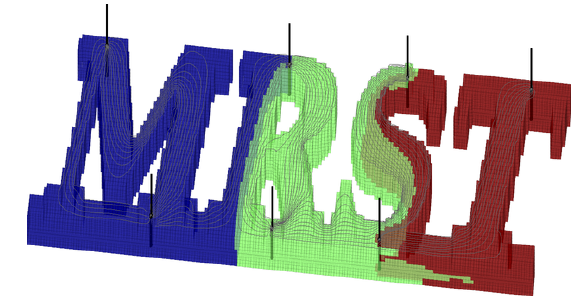
\includegraphics[width = 0.6\textwidth]{figures/misc/mrstlogo}
    \end{figure}
     \begin{textblock}{9.5}(6,10)
    MRST: Rapid prototyping of reservoir simulation models \cite{krogstad2015mrst}
  \end{textblock}

\end{frame}
}

{
\usebackgroundtemplate{\includegraphics[width = \textwidth, trim={-70 0 0 -140}, clip]{figures/misc/code}}
\begin{frame}
  \frametitle{MATLAB Reservoir Simulation Toolbox (MRST)}
  
  \begin{textblock}{9.5}(6,7)
    \begin{prettyList}
    \item \texttt{G}: geometric reservoir representation
    \item \texttt{rock}: petrophysical properties
    \item \texttt{fluid}: phase properties
    \item \texttt{model}: class defining residual equations, Jacobians, etc.
    \item \texttt{states}: reservoir properties at each time step
    \end{prettyList}
  \end{textblock}

\end{frame}
}

{
\usebackgroundtemplate{\includegraphics[width = \textwidth, trim={-70 0 0 -140}, clip]{figures/misc/code2}}
\begin{frame}
  
 \frametitle{MATLAB Reservoir Simulation Toolbox (MRST)}

 \begin{textblock}{10}(6,7)
    \begin{prettyList}
    \item Automatic differentiation
    \item Discrete versions of \texttt{Div}/\texttt{Grad}, no need to calculate Jacobians explicitly
    \item Write discrete equations on a form very similar to the semi-discrete:
      \begin{small}
        \begin{align*}
          \underbrace{\frac{1}{\Delta t} \big[(\phi b_o S_o)^{n+1}}_{\tikzmark{accum}} - (\phi b_o S_o)^{n}\big] + \underbrace{\nabla \cdot (b_o \vec v_o)^{n+1}}_{\tikzmark{flux}}
        \end{align*}
        \begin{tikzpicture}[remember picture,overlay]
          \draw [bend left, <-, line width = 1pt]($({pic cs:accum})+(0,6pt)$) - ++(-0em,-1.5ex)
          node[rectangle, draw, rounded corners, ultra thin, anchor=north,font=\small, align = center, fill = ye!10]
          {\scriptsize \texttt{(op.pv/dt).*pvMult.*bO.*sO}};
          \draw [bend left, <-, line width = 1pt]($({pic cs:flux})+(0,6pt)$) - ++(-0em,-2.4ex)
          node[rectangle, draw, rounded corners, ultra thin, anchor=north,font=\small, align = center, fill = ye!10]
          {\scriptsize \texttt{op.Div(bOvO)}};
          % \draw [<-, line width = 1pt]($({pic cs:krgT})+(0,6pt)$) |- ++(1em,-3.3ex)
          % node[rectangle, anchor=west,font=\small, text width = 2.5cm, align = center, fill = ntnublue!20]
          % {\scriptsize Total gas relperm};
        \end{tikzpicture}%
      %   \begin{align*}
      %   & \frac{1}{\Delta t} \left[(\phi b_o S_o)^{n+1} - (\phi b_o S_o)^{n}\right] + \nabla \cdot (b_o \vec v_o)
      %   & \text{\texttt{(op.pv/dt).*(pvMult.*bO.*sO }} \\ & \text{\texttt{- pvMult0.*bO0.*sO0) + op.Div(bOvO)}}
      % \end{align*}
    \end{small}
    \end{prettyList}
  \end{textblock}
    
\end{frame}
}


\section{Examples}

\begin{frame}
  \frametitle{Outline}
  \tableofcontents[currentsection]
\end{frame}


\begin{frame}
  \frametitle{Example 1: 1D displacement}
  \only<1>{
    \begin{prettyList}
    \item Initial saturation: $S_o = S_{or,i} = 0.2$, $S_w = 1 - S_{or, i}$
    \item Miscible residual saturation: $S_{or,m}= 0$
    \item Mixing: moderate ($\omega = 2/3$) and full ($\omega = 1$)
    \item 10 WAG-cycles over 4 years, 1 PV injected per year
    \end{prettyList}
  }
  \only<2->{
    \begin{overlayarea}{\textwidth}{0.7\textheight}
      \only<2>{
        \begin{center}
          \begin{mybox}{Moderate mixing}{0.63\textheight}
            \begin{center}
              \movie[showcontrols, width = 1\textwidth]{\includegraphics[width = \textwidth]{figures/displacement1D/placeholder}}
              {figures/videos/displacement1D.avi}
            \end{center}
          \end{mybox}
        \end{center}
      }
      \only<3>{
        \centering
        \begin{mybox}{Full mixing}{0.63\textheight}
          \begin{center}
            \movie[showcontrols, width = 1\textwidth]{\includegraphics[width = \textwidth]{figures/displacement1D/placeholder}}
            {figures/videos/displacement1D_1.avi}
          \end{center}
        \end{mybox}
      }
    \end{overlayarea}
  }
\end{frame}

\begin{frame}
  \frametitle{Example 2: Layer of SPE10}
  \only<1>{
    \begin{figure}[h]
      \centering
      \subfloat[Permeability]{
        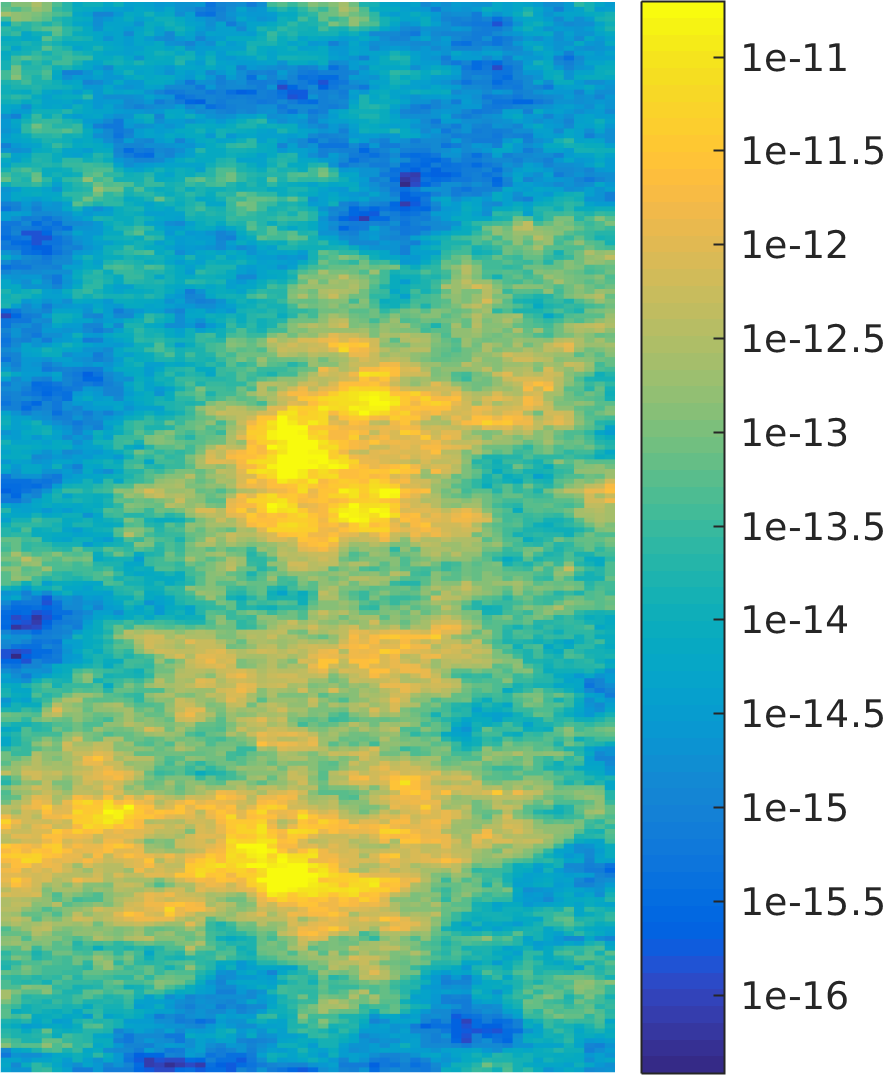
\includegraphics[height = 0.6\textheight]{figures/spe10/spe10perm}}\hspace{1em}
      \subfloat[Porosity]{
        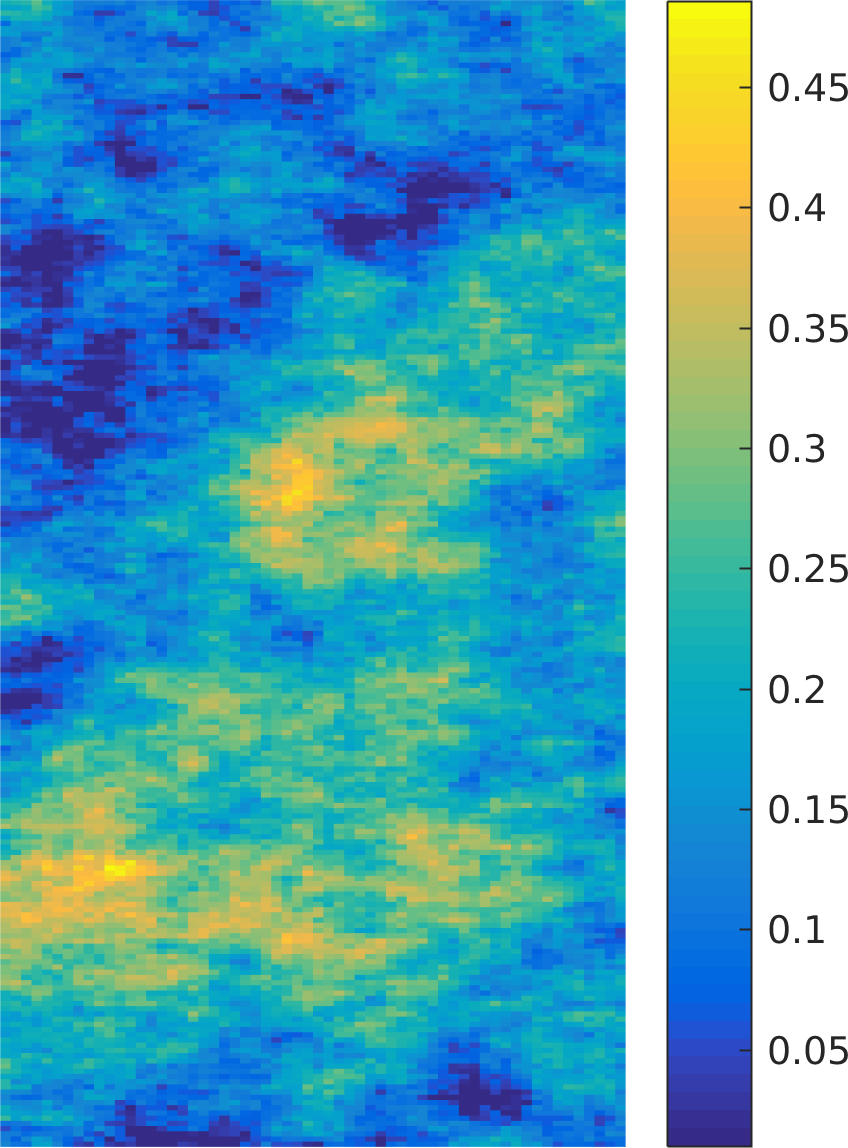
\includegraphics[height = 0.6\textheight]{figures/spe10/spe10poro}}
    \end{figure}
  }
  \only<2>{
    \begin{prettyList}
    \item Layer 10 of the SPE10 model \cite{spe10}, initially filled with oil
    \item Residual oil saturations: $S_{or,i} = 0.3$, $S_{or,m} = 0.0$
    \item Injection schedule:
    \end{prettyList}
    \begin{figure}[h]
      \centering
      \includegraphics[width = 0.9\textwidth]{figures/spe10/schedule}
    \end{figure}
  }
  \only<3>{
    \begin{center}
      \begin{mybox}{}{0.63\textheight}
        \vspace{0.2cm}
        \begin{center}
          \movie[showcontrols, width = 1\textwidth]{\includegraphics[width = \textwidth]{figures/spe10/placeholder}}
          {figures/videos/spe10_1.avi}
        \end{center}
      \end{mybox}
    \end{center}
  }
\end{frame}




\begin{frame}
  \frametitle{Example 2: Norne field model}
   \only<1>{
    \begin{figure}[h]
      \centering
      \subfloat[Permeability]{
        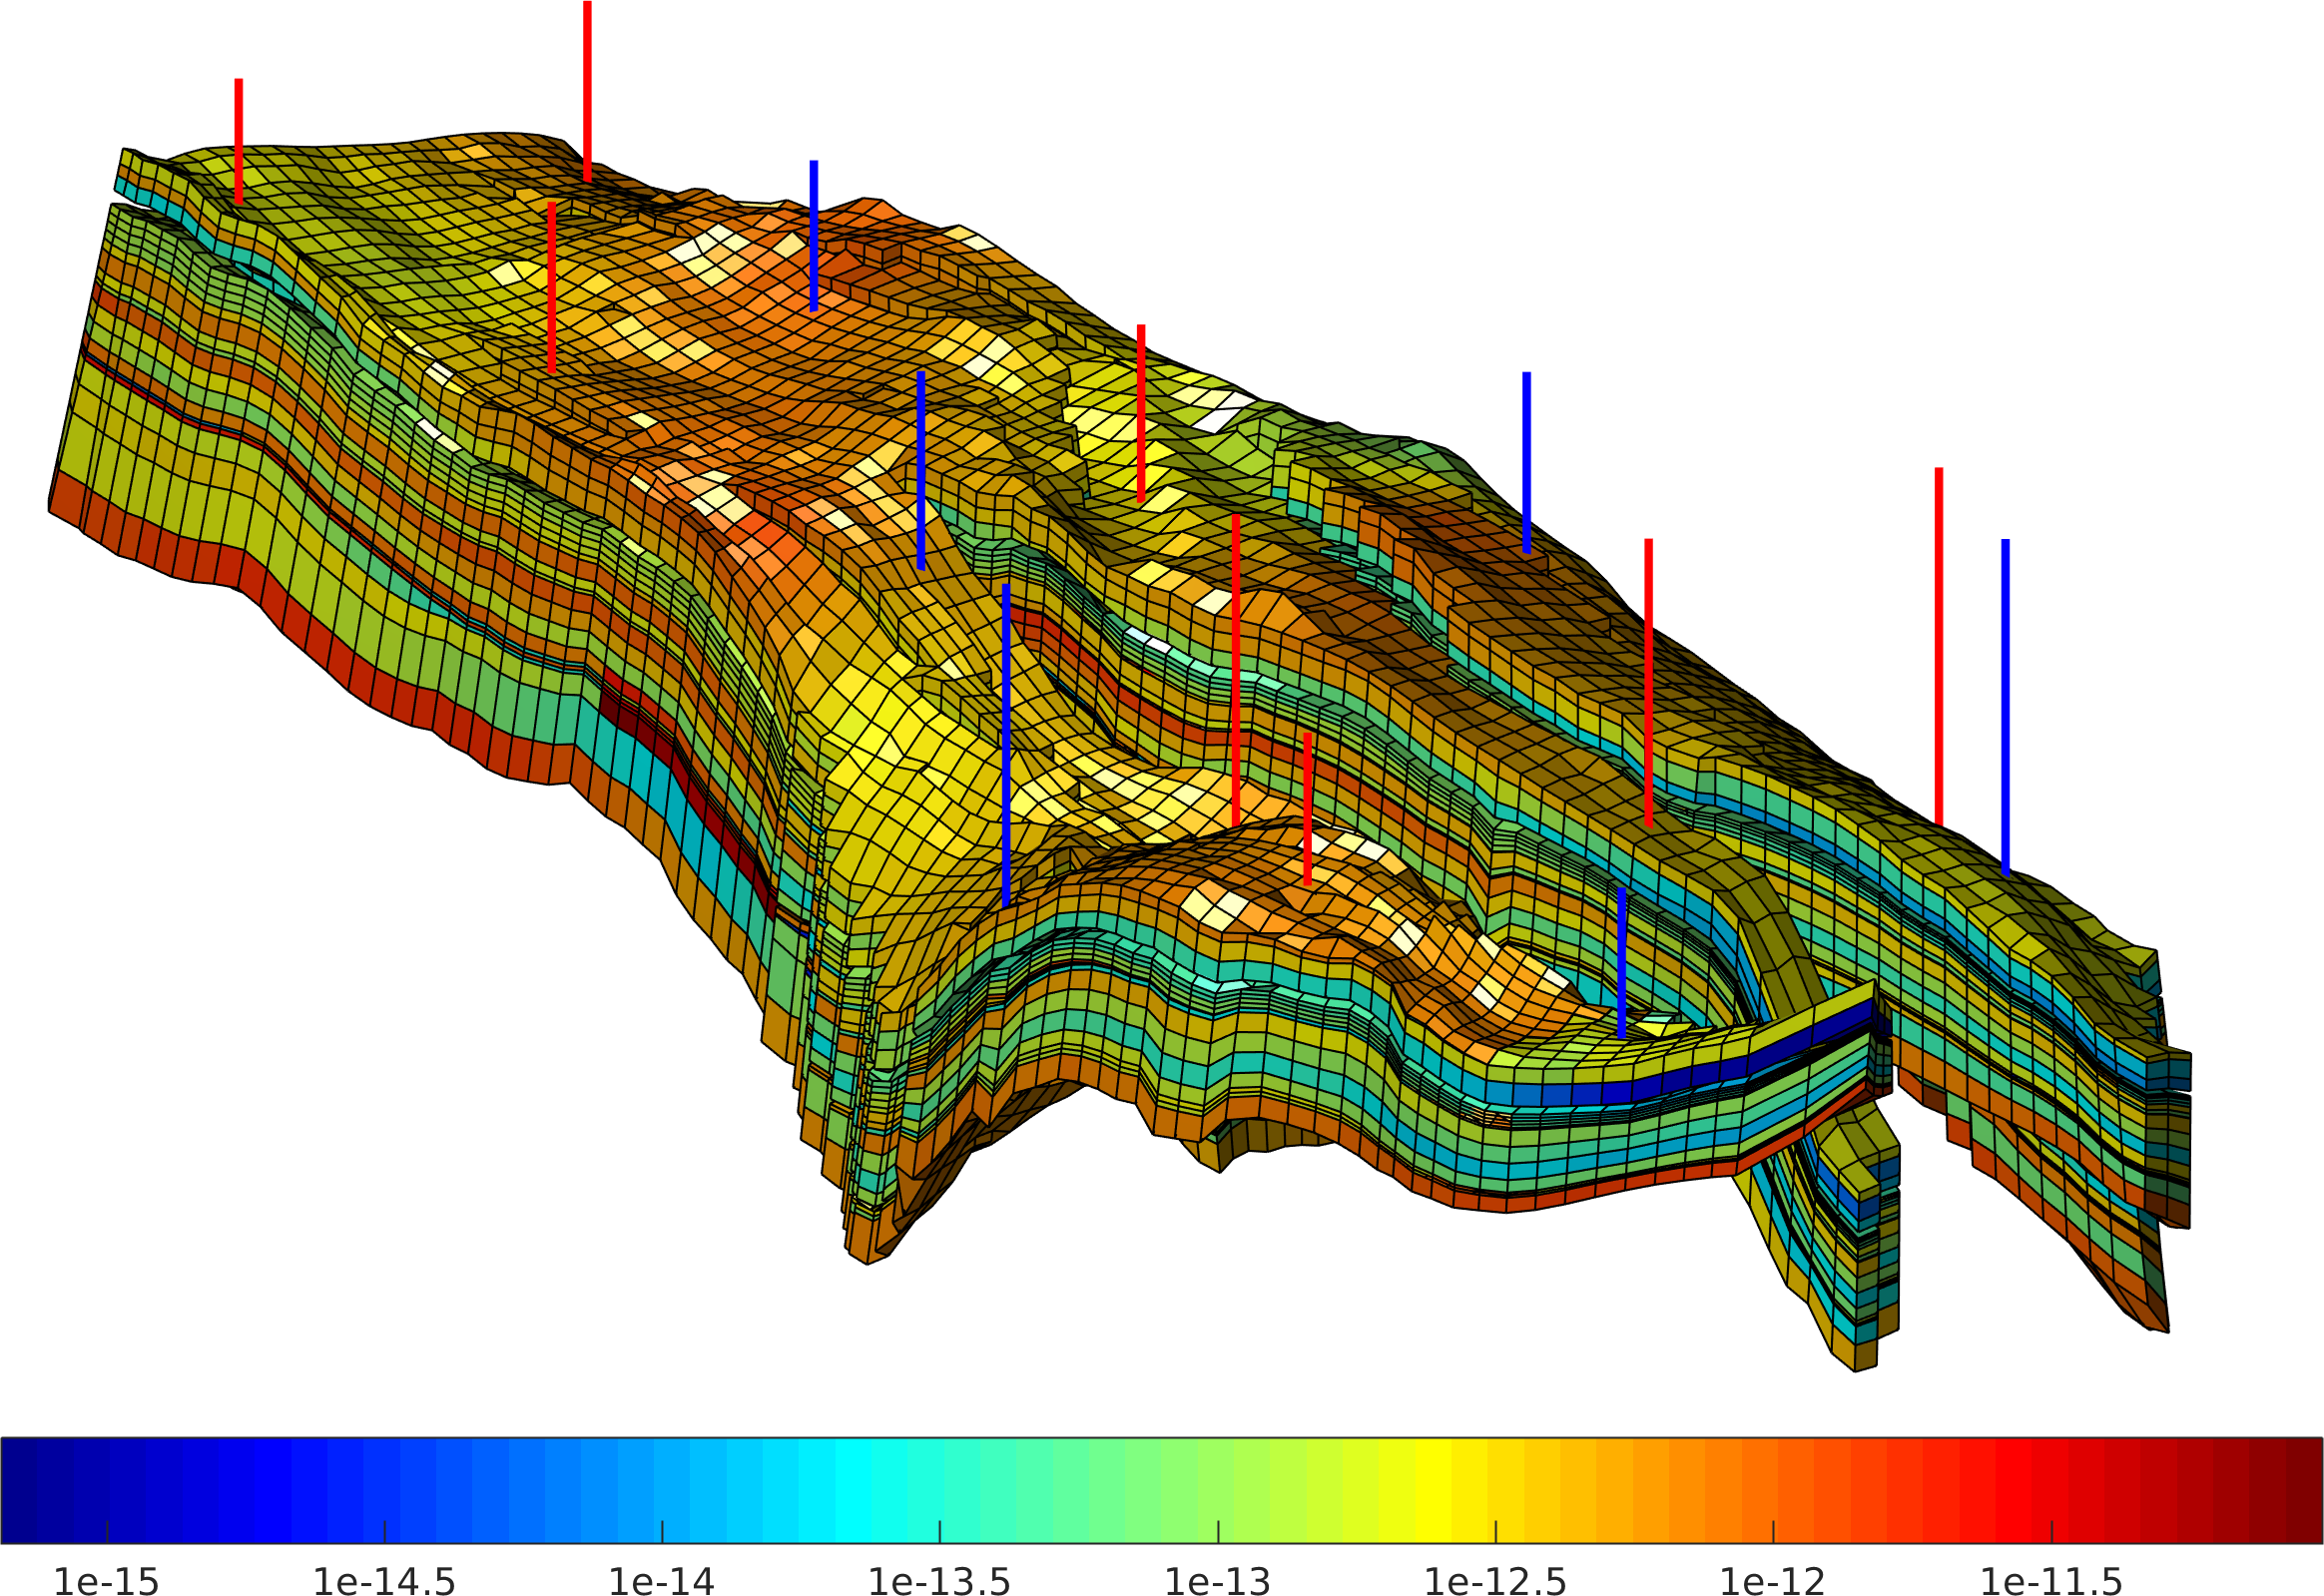
\includegraphics[width = 0.45\textwidth]{figures/norne/perm}}
      \subfloat[Porosity]{
        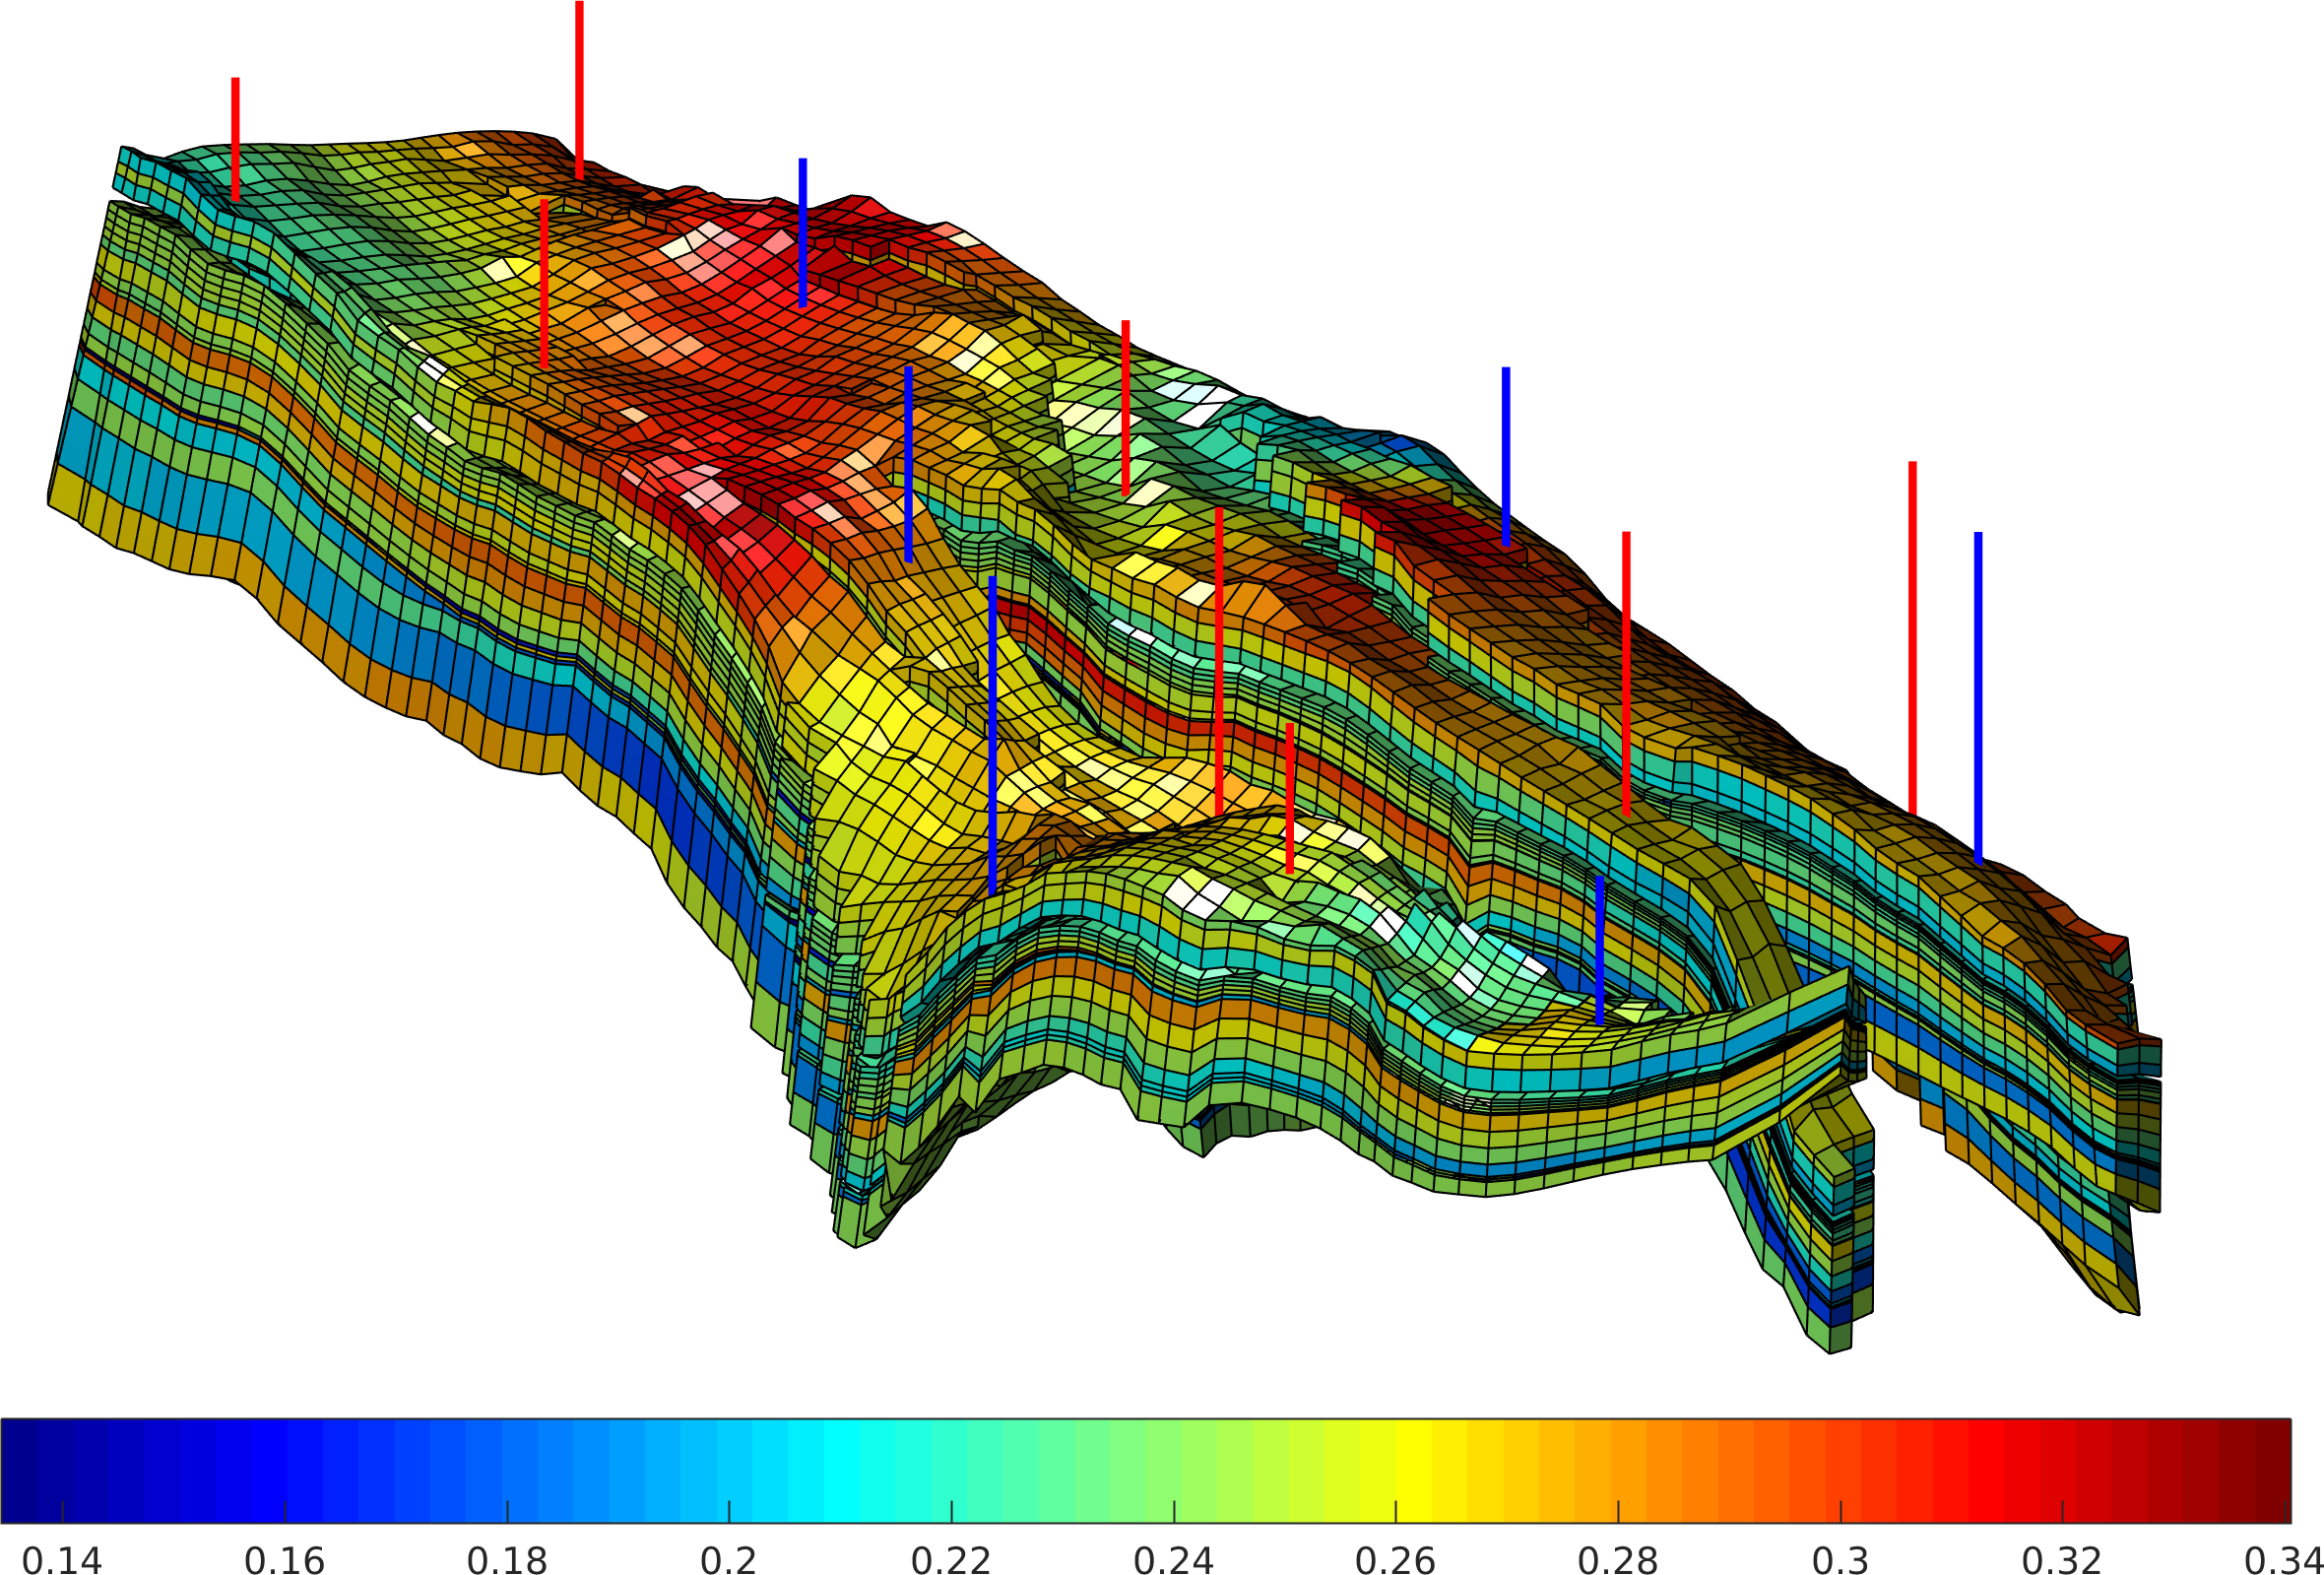
\includegraphics[width = 0.45\textwidth]{figures/norne/poro}}
    \end{figure}
    \begin{prettyList}
    \item Realistic field model \cite{norne-data} with $44,420$ cells, initially filled with oil
    \item Residual oil saturations: $S_{or,i} = 0.38$, $S_{or,m} = 0.08$
    \item Injection schedule:\\ \hspace{5ex}Large water slug -- 5 WAG cycles -- Small water slug
    \end{prettyList}
  }
  \only<2>{
    \begin{center}
      \begin{mybox}{}{0.65\textheight}
        \vspace{0.2cm}
        \begin{center}
          \movie[showcontrols, width = 1\textwidth]{\includegraphics[width = \textwidth]{figures/norne/placeholder}}
          {figures/videos/norne.avi}
        \end{center}
      \end{mybox}
    \end{center}
  }
  \only<3>{
    \begin{figure}[h]
      \centering
      \begin{tikzpicture}
        \node[anchor=south west,inner sep=0] at (0,0) {
      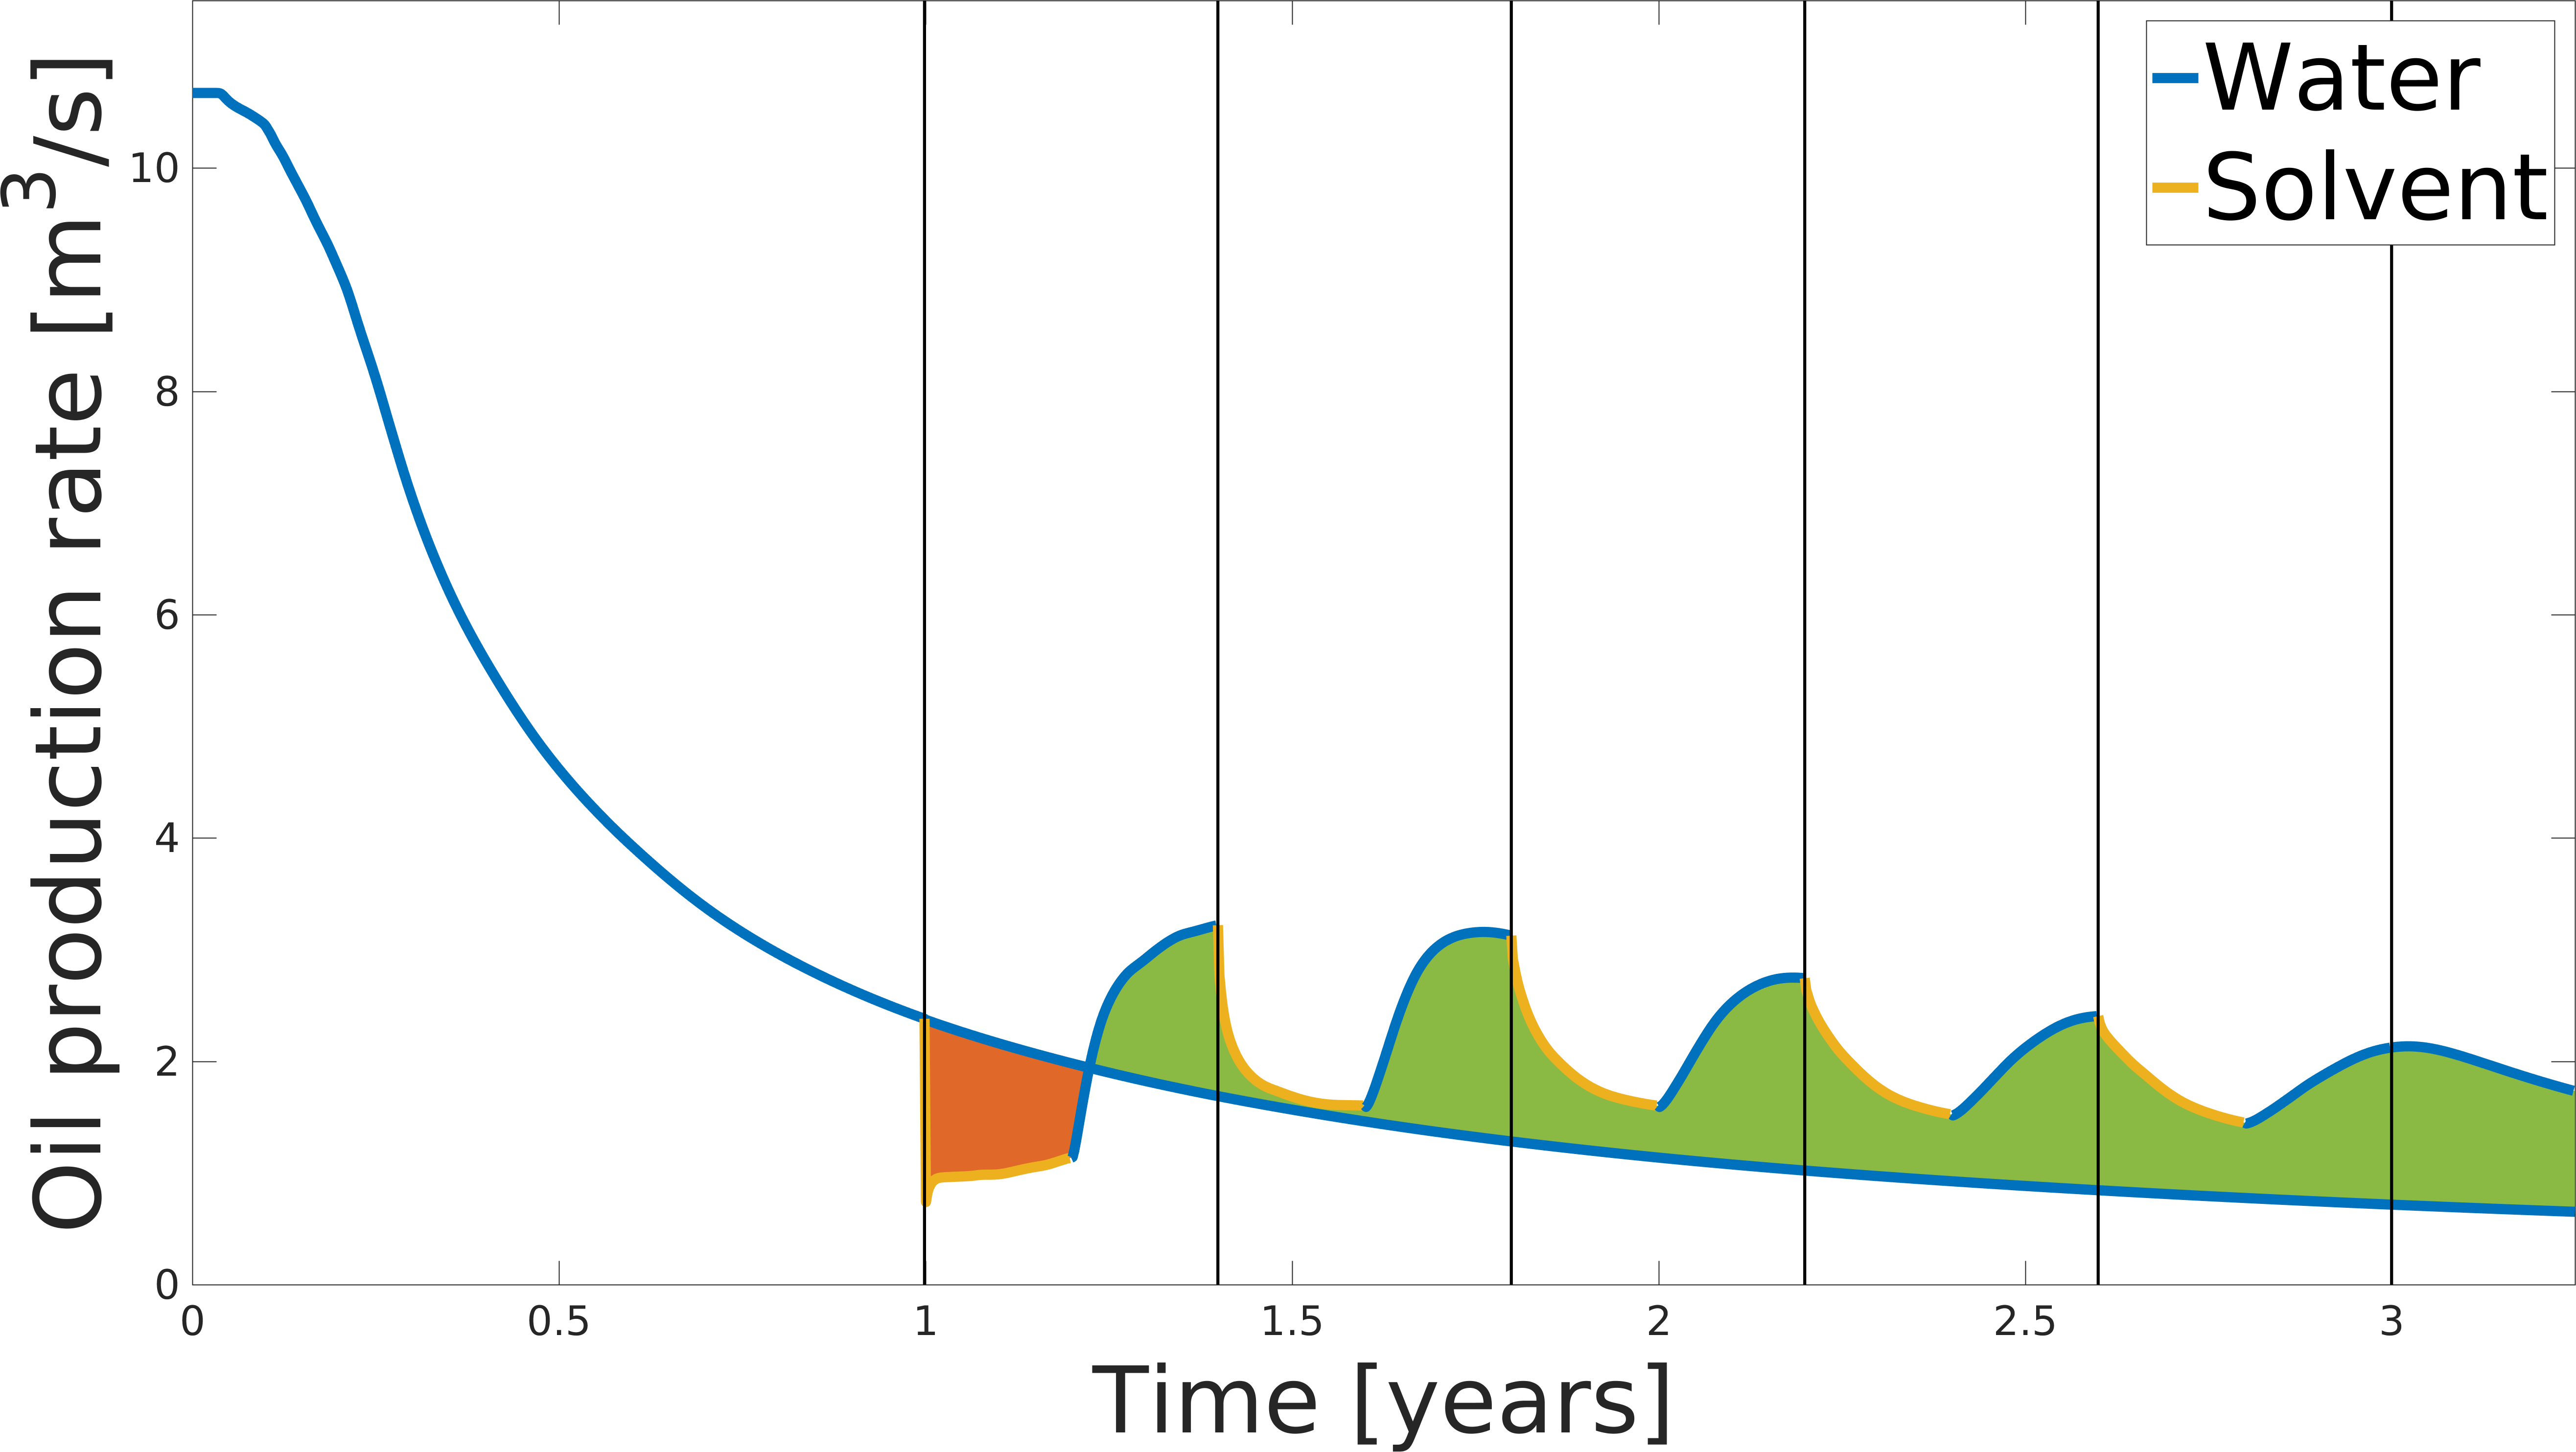
\includegraphics[width = 0.8\textwidth]{figures/norne/norneProduction}};
    \node[anchor = south, rectangle, draw, rounded corners, color = black, fill = white] (ir) at (4.5,3) {Increased recovery: 22 \%};
    \draw[-latex', line width = 1.5pt ] (ir.south) to[out = -90, in = 120] (5.3,1.5);
    \node at (3.8,5.3) {\tiny WAG 1};
    \node at (4.85,5.3) {\tiny WAG 2};
    \node at (5.9,5.3) {\tiny WAG 3};
    \node at (6.95,5.3) {\tiny WAG 4};
    \node at (8.0,5.3) {\tiny WAG 5};
      \end{tikzpicture}
    \end{figure}
  }
\end{frame}

\section{Conclusion and further work}

\begin{frame}
  \frametitle{Conclusion and further work}
  Conclusion
  \begin{prettyList}
  \item Implementation of a four-phase solvent model in MRST
  \item Able to simulate solvent injection on field-scale reservoir models
  \end{prettyList}\vspace{0.5cm}
  Further work
  \begin{prettyList}
  \item Validate model with ECLIPSE
  \item Implementation of higher-order FV methods
  \end{prettyList}
\end{frame}

\begin{frame}
  \frametitle{References}
  \begin{scriptsize}
    \bibliography{refs}
  \end{scriptsize}
\end{frame}

\end{document}


%%% Local Variables:
%%% mode: latex
%%% TeX-master: t
%%% End:
